\begin{enumerate}
	\item Exercício retirado da página 1023 de \cite{James_Stewart_calculo_v2}
	
	Calcule a integral abaixo, onde E está contido entre as esféras dadas abaixo no 1º octante.
	
	\begin{equation*}
		\iiint_E z\, dv
	\end{equation*}	
	\begin{equation*}
		E = \{(x,y,z) \,|\, 1 \leq x^2 + y^2 + z^2 \leq 4\}
	\end{equation*}
	
	\begin{figure}[htb]
		\caption{Coordenadas esféricas - Aula 06 - Exercício I}
		\label{v23_a06_e01}
		\centering
		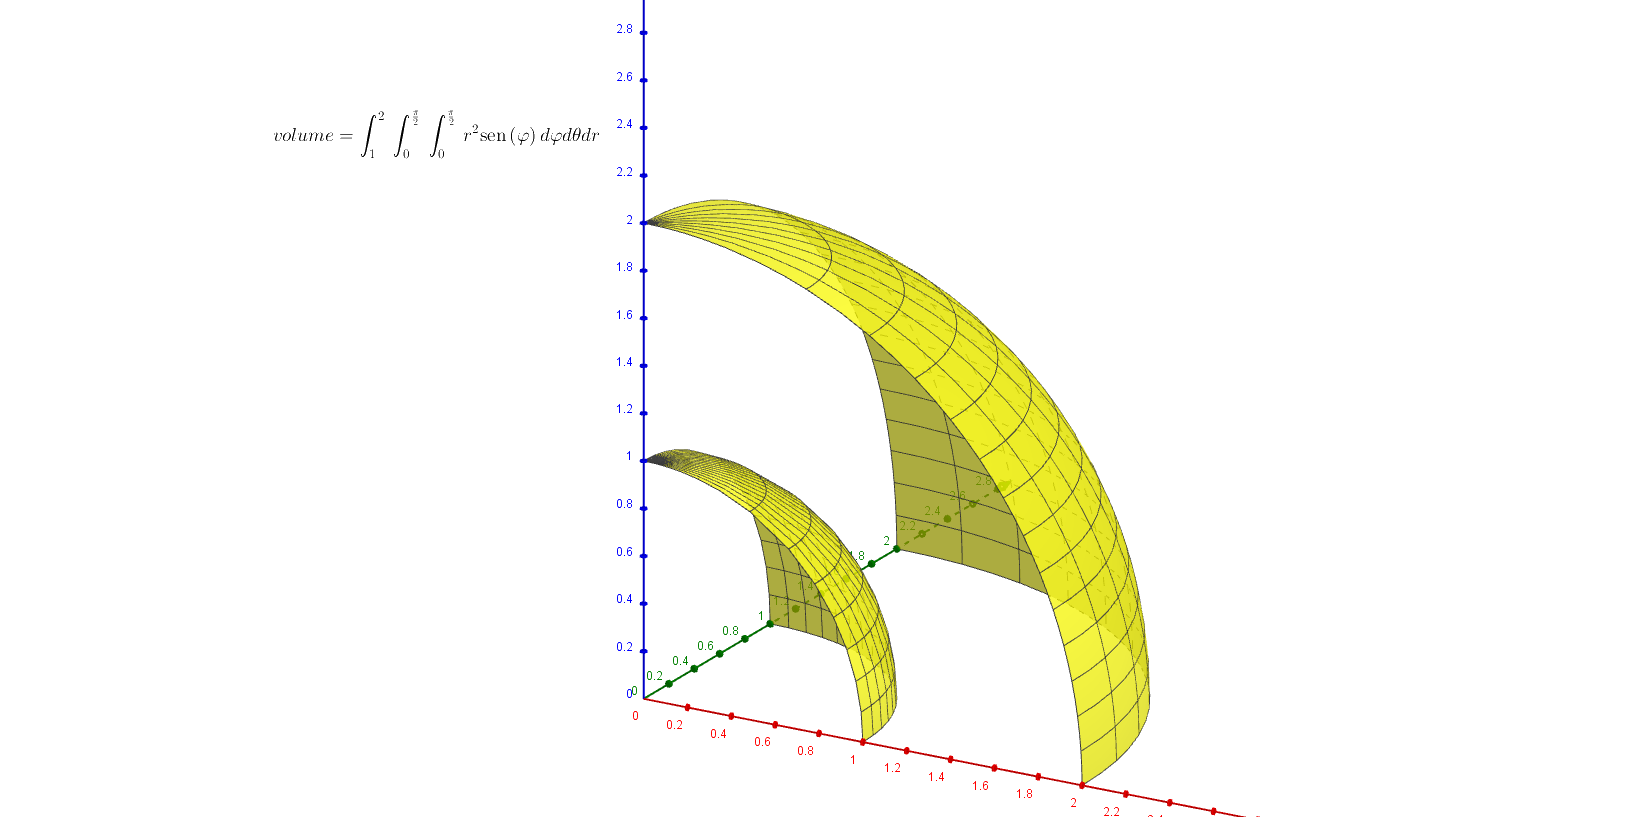
\includegraphics[width=0.5\textwidth]{v23_a06_e01.png}		
	\end{figure}
	
	\begin{equation*}
		z = r\cos(\varphi)
	\end{equation*}
	\begin{equation*}
		dv = dxdydz = r^2\sen(\varphi)\, dr d\theta d\varphi
	\end{equation*}                                    
	\begin{equation*}
		1 \leq r \leq 2,\, 0 \leq \theta \leq \dfrac{\pi}{2},\, 0 \leq \varphi \leq \dfrac{\pi}{2}
	\end{equation*}
	\begin{gather*}
		\iiint_E z\, dv = \int_1^2 \int_0^{\frac{\pi}{2}} \int_0^{\frac{\pi}{2}} \left(r\cos(\varphi)\right)r^2\sen(\varphi)\, d\varphi d\theta dr =\\ \int_1^2 r^3\, dr \int_0^{\frac{\pi}{2}} d\theta \int_0^{\frac{\pi}{2}} \sen(\varphi)\cos(\varphi)\, d\varphi = \left[\dfrac{r^4}{4}\right]_1^2 \left[\theta\right]_0^{\frac{\pi}{2}} \int_0^{\frac{\pi}{2}} u\, du = \left(\dfrac{16}{4} - \dfrac{1}{4}\right)\dfrac{\pi}{2}\left[\dfrac{u^2}{2}\right]_0^{\frac{\pi}{2}} =\\ \dfrac{16 - 1}{4}\dfrac{\pi}{2}\left[\dfrac{\sen^2(\varphi)}{2}\right]_0^{\frac{\pi}{2}} = \dfrac{15\pi}{16}\left[\sen^2\left(\dfrac{\pi}{2}\right) \overstrike{- \sen(0)}\right] = \dfrac{15\pi}{16}
	\end{gather*}
	\begin{equation*}
		u = \sen(\varphi) \Rightarrow du = \cos(\varphi)\, d\varphi
	\end{equation*}	
\end{enumerate}